\documentclass[a4paper,12pt]{article}

\usepackage{../usfdvl}


\title{Worksheet 1}
\SetDocumentFooter{}{}


\begin{document}

\maketitle


\vspace{5pt}
\section{Ground Rules}

\myparagraph{This assignment is intended to be done alone. You may ask others for high-level help. However, the answer must be yours.}

\vspace{5pt}
\section{Assignment}

\begin{enumerate}
\item Does $2^{n+1}=O(2^n)$? If not, what does it equal?

\item Does $2^{2n}=O(2^n)$? If not, what does it equal?

\item Prove by mathematical induction that the following formula, $3^2+3^3+...3^n=9\left( \frac{3^{n-1}-1}{2} \right)$, holds for $\forall \geq 2$.

\item Determine whether the orientation of the following triangles (show your work).


\begin{itemize}
\item $\{\{2,3\},\{5,6\},\{3,5\}\}$
\item $\{\{3,2\},\{1,6\},\{4,4\}\}$
\item $\{\{1,4\},\{5,6\},\{9,8\}\}$
\end{itemize}


\item Show the 10 iterations of the line sweep algorithm on the following set of segments. At each step show the event queue, segment order, and indicate which segments are compared for intersection.

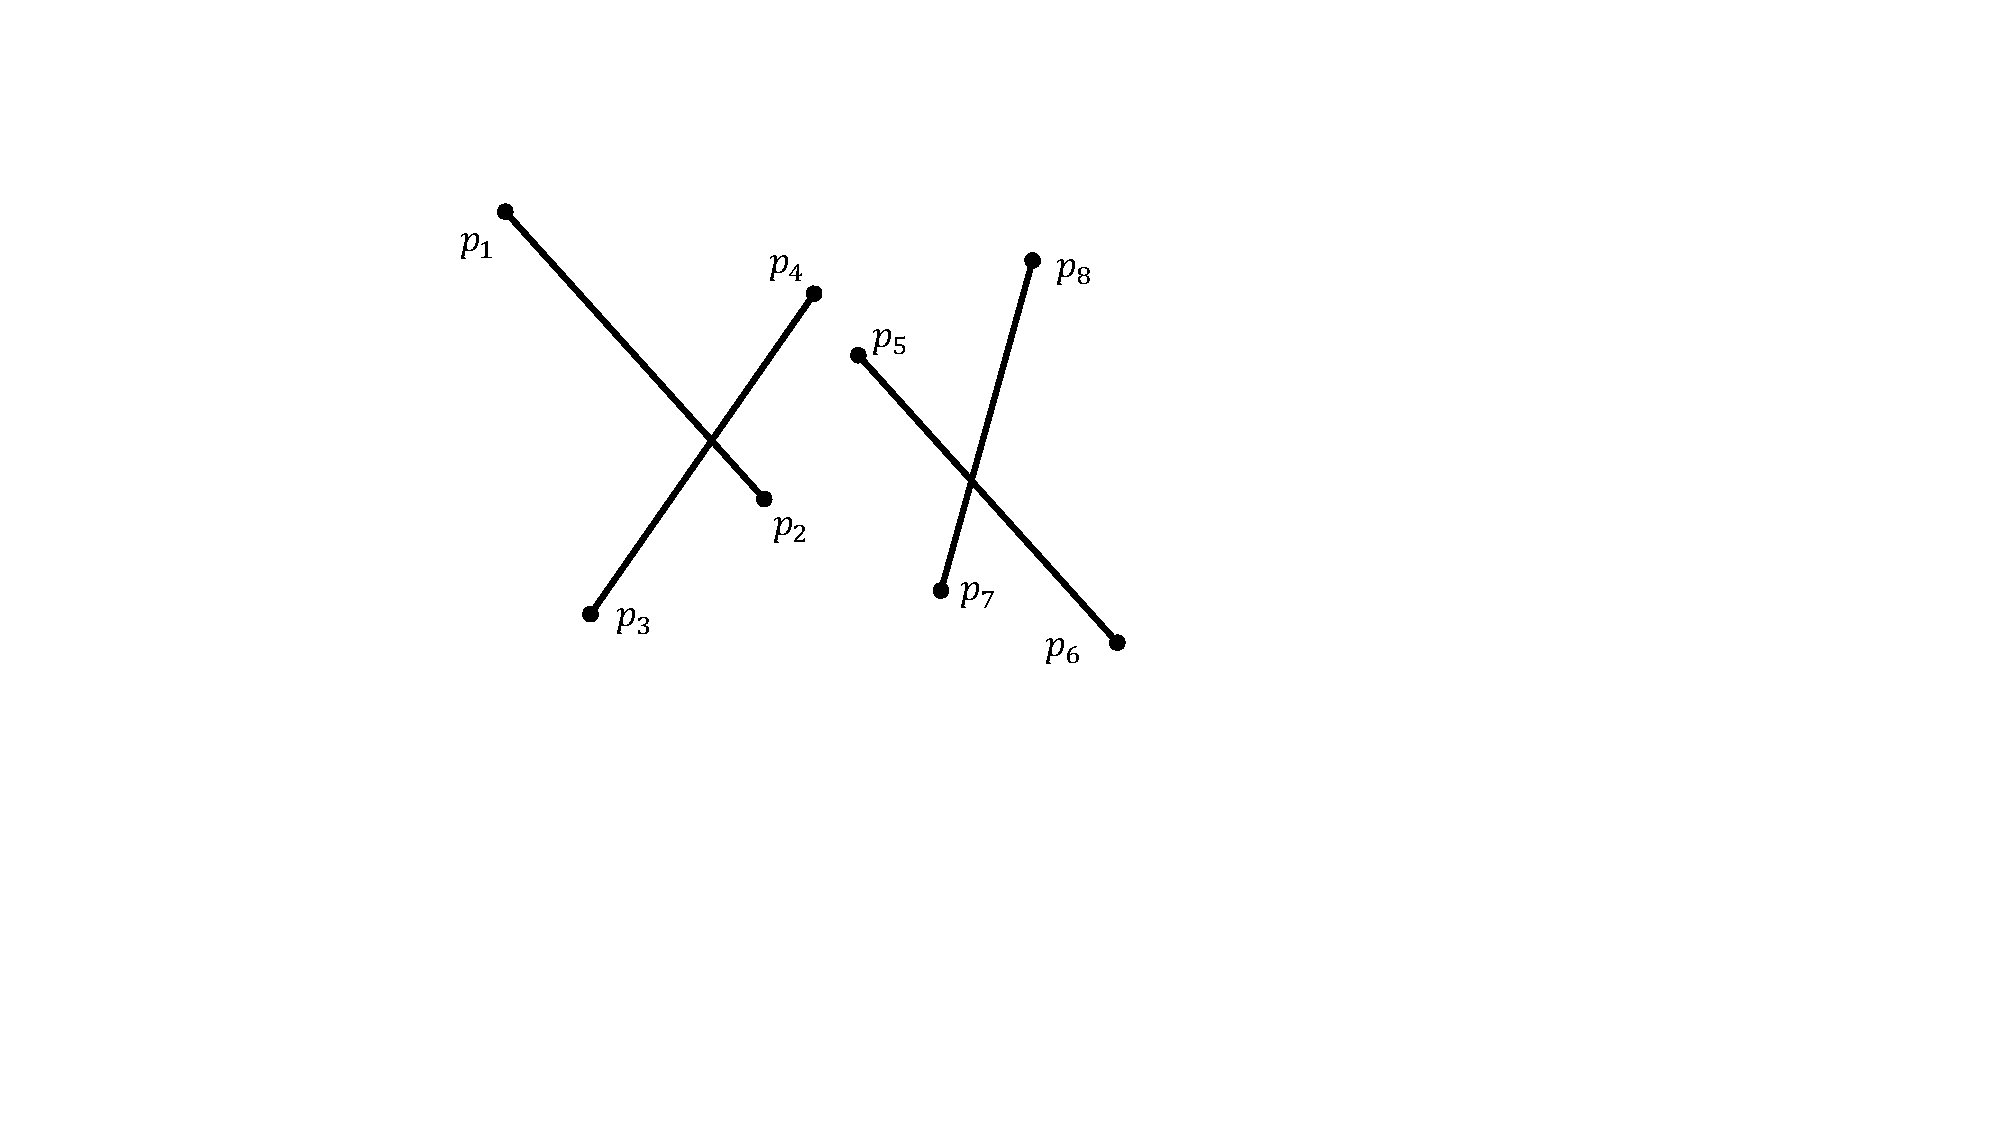
\includegraphics[width=7cm]{../images/linesweep.pdf}
\end{enumerate}


\section{Submission}

\myparagraph{Upload your answers and associated work to canvas as a single scanned, types, or photographed PDF document. Be sure that your submission is legible.}



\end{document}
